\section{Perturbation Analysis}

We explored two related methods for analysing transfer in progressive networks.
One based on Fisher information yields the Average Fisher Sensitivity (AFS)
and is described in Section 3 of the paper. We describe
the second method based on perturbation analysis in this appendix, as it proved
too slow to use at scale. Given its intuitive appeal however, we provide
details of the method along with results on Pong Variants (see
Section 5.2), as a means to corroborate the AFS score.

Our perturbation analysis aims to estimate which components of the source
columns materially contribute to the performance of the final column on the
target tasks. To this end, we injected Gaussian noise into each of the (post-ReLU) hidden
representations, with a new sample on every forward pass, and calculated the
average effect of these perturbations on the game score over 10 episodes.  We
did this at a coarse scale, by adding noise across all features of a given
layer, though a fine scale analysis is also possible per feature (map).
In order to be invariant to any arbitrary scale factors in the network weights,
we scale the noise variance proportional to the variance of the activations in
each feature map and fully-connected neuron. Scaling the variance in this
manner is analogous to computing the Fisher w.r.t. normalized activations for
the AFS score.

\begin{figure}[h]
  \centering
    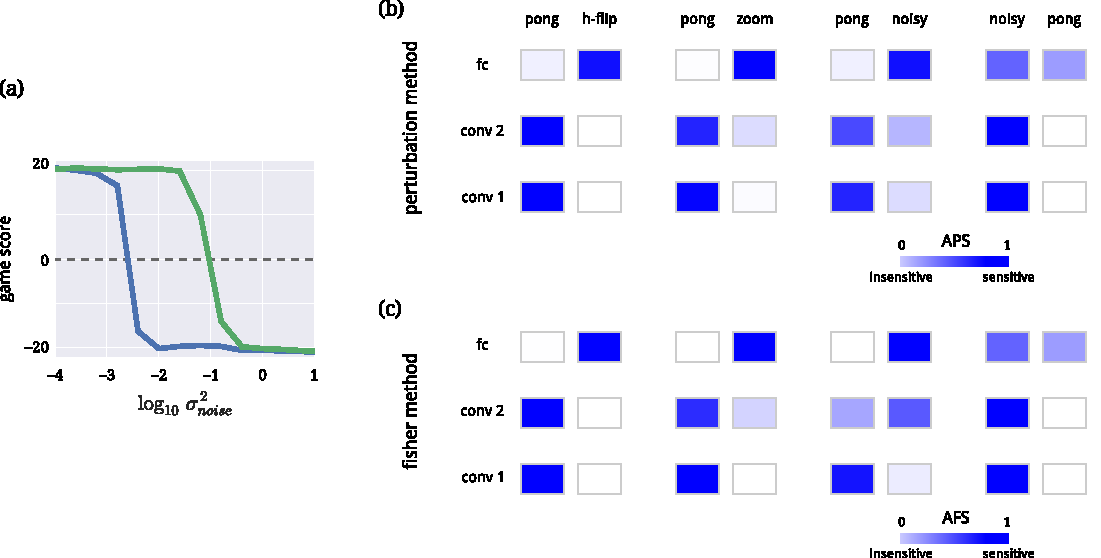
\includegraphics[width=.95\textwidth]{figures/appendix_AFS_vs_APS.pdf}
    \caption{(a) Perturbation analysis for the two second-layer
      convolutional representations in the two columns of the
      Pong/Pong-noise net. Blue: adding noise to second convolutional layer from column 1;
      green: from column 2. Grey line determines critical noise
      magnitude for each representation, $\sigma_i^2$.
      (b-c) Comparison of per-layer sensitivities obtained using the APS
      method (b) and the AFS method (c; as per main text).
      These are highly similar.}
    \label{fig:app_afs_vs_aps}
\end{figure}

Define ${\Lambda_i^{(k)}}=1/\sigma_i^{2(k)}$ as the precision of the noise
injected at layer $i$ of column $k$, which results in a $50\%$ drop in
performance. The Average Perturbation Sensitivity (APS) for this layer is
simply:
\begin{align}
    \text{APS}(i,k) = \frac{\Lambda_i^{(k)}}{\sum_k \Lambda_i^{(k)}}
\end{align}
Note that this value is normalized across columns for a given layer. The APS
score can thus be interpreted as the responsibility of each column in a given
layer to final performance.
The APS score of 2-column progressive networks trained on Pong Variants is
shown in Fig\ref{fig:app_afs_vs_aps} (b). These clearly corroborate the
AFS shown in (c).
